\documentclass[12pt]{article}

\usepackage[margin=1.0in]{geometry}
\usepackage{graphicx}
\usepackage{listings}
\usepackage{tabto}
\graphicspath{ {./} }


\begin{document}

\title{CS4347 : Database SystemsHomework Assignment 3}
\author{Matthew McMillianmgm160130@utdallas.edu}
\maketitle



\begin{enumerate}
	
	\item We can remodel the relationship between LOANS, ACCOUNTS, and TRANSACTIONS below using a specialization approach. 
		\begin{center}
			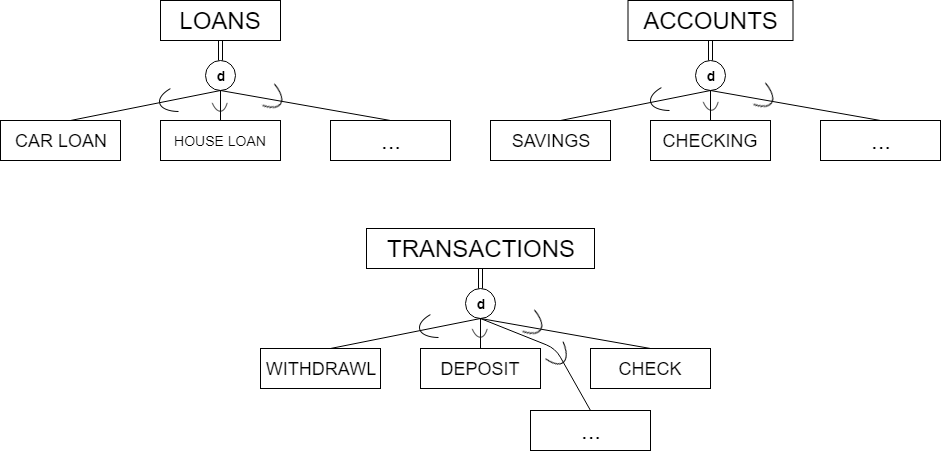
\includegraphics[scale=0.45]{eer3}
		\end{center} 
	In regards to the loan's attributes (date, time, amount), we can add those attributes onto the ACCOUNTS table, since all of the loan types will inherit those values. In this example, we are assuming that there are not many (if any) special attributes, but if there were we would need to add their respective attributes to the EER. We can view this as a generalization since we are lacking information regarding the attributes needed (if any) for each subclass, but if we had more information about the database we could consider this a specialization. If we wanted to, we could define subtables for each of the tables listed and treat it's superclass as a generalization of those classes. However, if we add distinct features to each 'special' class we could consider this as a specialization example since each child would be a specialization of the superclass. If it turns out that the subclasses have greater attributes  than the superclass, I think it would be better to consider this a generalization case since the subclasses would be very detailed compared to its 'general' parent.
	\pagebreak
	\item The integrity constraints violated or concerns are listed below:
	\begin{itemize}
		\item[(a.)] The insert needs to update all foreign key values from values in the employee table. In this case, WORKS$\_$ON would need to be updated with the employee's ESSN foreign key (we will discuss the other foreign key issue later). Any DEPENDENTS of the employee would need to be inserted as well (or updated) with the new ESSN, if updated.
		\item[(b.)] Since (b.) is a new project, no updating needs to be done and no constraints in this case are violated.
		\item[(c.)] Case (c.) violated a key constraint since it is attempting to override Administration as department number '4'. If the insert is meant to update without changing anything, it would be OK to do this. However, if we wanted to conserve the integrity of the the other teams/projects, we would either have to reassign the keys in all those tables which would be horrible. Ideally we would throw and error at the insert and have the insert query change its department key. Even still if we did this would would have to update the DEPT$\_$LOCATIONS relationship table.
		\item[(d.)] Case (d.) violated the Pno NOT NULL relationship. This should throw and error and have the person inserting this value add a project number.
		\item[(e.)] This insert should be OK since it has a valid foreign key, and nothing in dependent requires other tables to be updated.
		\item[(f.)] If an employee HAS to work on a project, then this would violate the condition that each employee needs to work on a project which should result in an error violating the constraint. If an employee does NOT have to work on a project, this would be OK since WORKS$\_$ON does not affect tables outside of itself.
		\item[(g.)] Deleting the employee tuple would violate many constraints. You would have to m ake sure that if you delete the employee, all foreign keys (the rows of the foreign keys) for ESSN in WORKS$\_$ON and DEPENDENT would need to be deleted. Also, if the employee manager of a department, one would need to be reassigned.
		\item[(h.)] Deleting this project would violate many constraints. Since that Pno is referenced in many other tables, any other rows in the other tables with foreign key Pno would need to be deleted as well. If there are any constraints about having more than one project being worked on, etc., those constraints would also be violated and an error would need be thrown.
		\item[(i.)] Since no other tables depend on Mgr$\_$ssn and Mgr$\_$start$\_$date, it is OK to change these values.
		\item[(j.)] As long as the Super$\_$ssn meets the constraints that the employee must be a supervisor, then the change is OK. If not, then it should throw and error.
		\item[(k.)] Since HOURS has no other attribute that it's dependent on, we can change hours with no problem.
	\end{itemize}
	\pagebreak
	\item The integrity constraints for figure 1.2 are listed below:
	\begin{itemize}
		\item[(a.)] Referential constraints that hold for this schema are the section$\_$numbers, course$\_$numbers w/ prerequisite$\_$number, and student$\_$numbers since they all hold relations across multiple tables.
		\item[(b.)] The appropriate DDL commands to define the database are given below: 
\begin{center}
\begin{lstlisting}[language=sql]
CREATE TABLE STUDENT (
	Name			VARCHAR(15) 	NOT NULL, 
	Student_number 		VARCHAR(15) 	NOT NULL, 
	Class			VARCHAR(15) 	NOT NULL,
	Major			VARCHAR(15)
); 			
			
CREATE TABLE COURSE (
	Course_name		VARCHAR(15)	NOT NULL,
	Course_number 		VARCHAR(8) 	NOT NULL,
	Credit_hours		NUMBER 		NOT NULL,
	Department		VARCHAR(4)
); 
			
CREATE TABLE SECTION (
	Section_identifier 	NUMBER		NOT NULL,
	Course_number 		VARCHAR(8) 	NOT NULL,
	Semester		VARCHAR(8) 	NOT NULL,
	Year			NUMBER		NOT NULL
); 
			
CREATE TABLE GRADE_REPORT (
	Course_number		VARCHAR(8)  	NOT NULL,
	Prerequisite_number 	VARCHAR(8)  	NOT NULL
);
\end{lstlisting}
\end{center}
		
	\end{itemize}
\end{enumerate}


\end{document}
